
\documentclass[11pt]{article}
\usepackage[a4paper,margin=1in]{geometry}
\usepackage{amsmath,amssymb,amsthm}
\usepackage{mathtools}
\usepackage{microtype}
\usepackage{booktabs}
\usepackage{enumitem}
\usepackage{hyperref}
\usepackage{tikz}
\usetikzlibrary{arrows.meta,positioning,fit}

\title{\textbf{Executable Commitment Theory (ECT)}\\\large A programmatic complement to game theory}
\date{} % no date
\author{} % intentionally blank

\newtheorem{definition}{Definition}
\newtheorem{proposition}{Proposition}

\newcommand{\E}{\mathbb{E}}
\newcommand{\A}{A}
\newcommand{\Hhist}{H}
\newcommand{\PPi}{\Pi}
\newcommand{\DeltaD}{\Delta}
\newcommand{\Ui}{U_i}
\newcommand{\ui}{u_i}

\begin{document}
\maketitle

\begin{abstract}
Players do not only choose actions; they choose \emph{executable, verifiable policies}. What matters strategically is not just what one intends to do, but what one can \emph{publicly prove} their system will do under contingencies. In Executable Commitment Theory (ECT), credible commitments are endogenous, programmable, and checkable. This short note sketches the formal objects, introduces the equilibrium concept of \emph{Proof--Commitment Equilibrium} (PCE), works a 2$\times$2 example, and offers a conceptual figure.
\end{abstract}

\section*{Objects}
Consider a finite set of players $i=1,\dots,n$.
\begin{itemize}[leftmargin=1.2em]
  \item Each player chooses an \textbf{executable policy} $\pi_i \in \PPi_i$, where $\pi_i:\Hhist \to \DeltaD(\A_i)$ maps histories $\Hhist$ to mixed actions over $A_i$.
  \item A public \textbf{verifier} $V$ certifies selected properties $\phi_i$ of $\pi_i$ (e.g.\ a retaliation rule, an expenditure cap, or a worst-case response time bound).
  \item Certification may be \emph{selective}: others observe $\phi_i$ without seeing the code (\emph{e.g.}, via zero-knowledge or hardware attestation).
\end{itemize}

\paragraph{Costs and payoffs.}
Let $c(\pi_i)$ denote compute/maintenance cost and $\tau(\pi_i)$ a latency proxy. For state $s$ and action profile $a$, base utility is $\ui(a,s)$. Effective payoff is
\begin{equation}
  \Ui(\pi_1,\ldots,\pi_n)
  \;=\; \E[\ui(a,s)] - \lambda_i\, c(\pi_i) - \mu_i\, \tau(\pi_i).
\end{equation}

\paragraph{Admissibility.}
A policy $\pi_i$ is \emph{admissible} if $V(\pi_i,P)=\text{true}$ for its declared property set $P$ (it both satisfies and can prove its guarantees).

\begin{definition}[Proof--Commitment Equilibrium (PCE)]
A profile $(\pi_1,\ldots,\pi_n)$ with certificates $(\phi_1,\ldots,\phi_n)$ is a PCE if no player can switch to any \emph{admissible} policy $\pi_i'$ that yields a strictly higher $\Ui$ given others' certified properties. A \emph{ZK--PCE} further restricts certification to reveal only selected $\phi_i$ via zero-knowledge.
\end{definition}

\section*{Why ECT complements classical game theory}
\begin{itemize}[leftmargin=1.2em]
  \item Credible commitments become \emph{endogenous and programmable}; strategy sets expand from actions to \emph{policies-with-proofs}.
  \item New strategic resources emerge: \emph{commitment capital} (what you can prove), \emph{verification bandwidth}, and \emph{latency advantage}.
  \item PCE refines equilibrium selection when threats and promises are made verifiable.
\end{itemize}

\section*{Worked $2\times 2$ example: deterrence by executable commitment}
Two players choose between \textsc{Attack} (A) and \textsc{Wait} (W).
\begin{center}
\begin{tabular}{@{}lcc@{}}
\toprule
 & \textbf{Col: A} & \textbf{Col: W} \\
\midrule
\textbf{Row: A} & $(-2,-2)$ & $(3,-3)$ \\
\textbf{Row: W} & $(-3,3)$ & $(1,1)$ \\
\bottomrule
\end{tabular}\\[0.5em]
\emph{Baseline:} best response to A is A, to W is A $\Rightarrow$ unique Nash at (A,A).
\end{center}

Now let Column publish a certified policy ``auto-retaliate within $\le 1$ms if attacked.'' Given certification, Row's expected payoff from A against Column's W collapses (e.g.\ to $-10$ instead of $3$), selecting (W,W) under PCE:
\begin{center}
\begin{tabular}{@{}lcc@{}}
\toprule
 & \textbf{Col: A} & \textbf{Col: W (certified retaliation)} \\
\midrule
\textbf{Row: A} & $(-2,-2)$ & $(-10,-1)$ \\
\textbf{Row: W} & $(-3,3)$ & $(1,1)$ \\
\bottomrule
\end{tabular}
\end{center}

\section*{Conceptual figure (policy $\to$ proof $\to$ play)}
\begin{center}
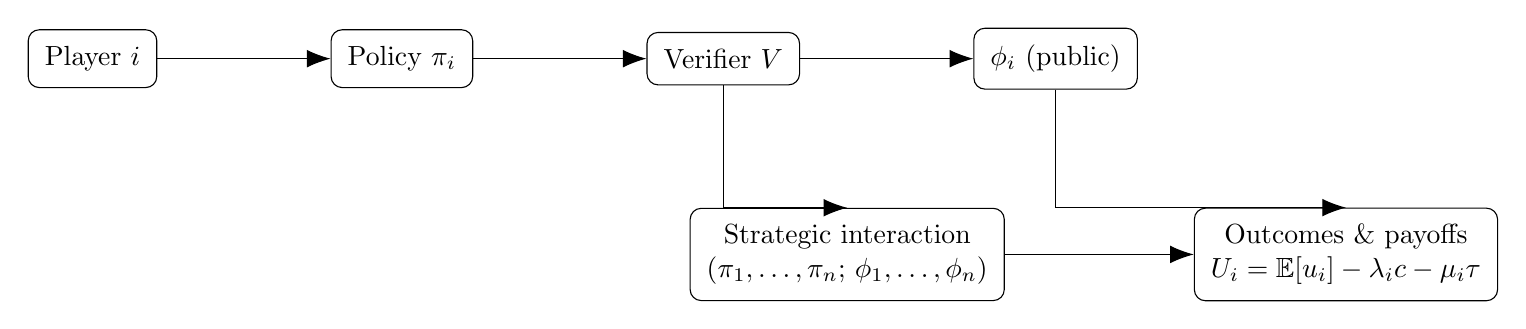
\begin{tikzpicture}[node distance=1.7cm]
\tikzset{box/.style={draw, rounded corners, align=center, inner sep=6pt}}
\node[box] (player) {Player $i$};
\node[box, right=2.2cm of player] (policy) {Policy $\pi_i$};
\node[box, right=2.2cm of policy] (verifier) {Verifier $V$};
\node[box, right=2.2cm of verifier] (props) {$\phi_i$ (public)};

\draw[-{Latex[length=3mm]}] (player) -- (policy);
\draw[-{Latex[length=3mm]}] (policy) -- (verifier);
\draw[-{Latex[length=3mm]}] (verifier) -- (props);

\node[box, below left=1.5cm and -0.4cm of props] (interaction) {Strategic interaction\\ $(\pi_1,\ldots,\pi_n;\,\phi_1,\ldots,\phi_n)$};
\node[box, right=2.4cm of interaction] (payoffs) {Outcomes \& payoffs\\ $\Ui=\E[\ui]-\lambda_i c-\mu_i \tau$};

\draw[-{Latex[length=3mm]}] (verifier.south) |- (interaction.north);
\draw[-{Latex[length=3mm]}] (props.south) |- (payoffs.north);
\draw[-{Latex[length=3mm]}] (interaction) -- (payoffs);
\end{tikzpicture}
\end{center}

\section*{Open questions}
\begin{itemize}[leftmargin=1.2em]
  \item Existence and characterization of PCE; relation to Nash and subgame perfection in induced program games.
  \item Complexity of best responses over policy spaces; approximation schemes.
  \item Revelation-principle analogues for proofs; optimal disclosure under verification bandwidth limits.
  \item Market design and auctions with verifiable bidding policies; multi-agent RL that learns in the space of \emph{policies+proofs}.
\end{itemize}

\end{document}
